
\newcommand{\figCaption}[1]{\paragraph{Figure \ref{#1}} [page \pageref{#1}]}
\newcommand{\figCaptionTwo}[2]{\paragraph{Figure \ref{#1}, \ref{#2}} [page \pageref{#1}, \pageref{#2}]}

\chapter{About figures}
\label{chap:aboutFigures}

All images of \lsystems in this thesis (if not stated otherwise) are created in the created web by written \lsystem processing library.
Some source codes in the thesis and may be simplified because of lack of the space.
This appendix contains additional information about figures and their source codes.

\figCaptionTwo{fig:introLilac}{fig:rsltLilac} 3D model of lilac panicle \cite[p.~92]{PL91}. 
Some blooms have 4 and some 5 leafs.

\begin{LsystemBreak}
lsystem LilacInflorescences extends Branches {	
	// A(energy, branchEnergy)
	set symbols axiom = F(50) A(12, 5);
	set iterations = 12;

	interpret F as DrawForward(10, 2, #00AA00);
	interpret K(age) as lsystem Bloom(age);
	interpret + as Pitch(60);
	interpret - as Pitch(-60);
	interpret / as Roll(90);

	rewrite A(energy) where energy <= 0 to K(1);
	rewrite A(energy, branchEnergy) to [ - / K(1) ] [ + / K(1) ]
		I(0, branchEnergy) / A(energy - 1, branchEnergy);
	rewrite I(t, energy) where energy <= 0 to nothing;
	rewrite I(t, energy) with e = energy - 1, be = energy where t==2
		to I(t + 1, e) [ - F F A(e, be) ] [ + F F A(e, be) ];
	rewrite I(t, e) to F I(t + 1, e - 1);
	rewrite K(age) to K(age + 1);
}
abstract lsystem Bloom(age = 4) extends Polygons {
	let color = #d649ff;
	let leafCount = round(random(3.5, 5.5));
	let angle = 150 / leafCount;
	let size = min(4, age);

	set symbols axiom = F [ G(1.5) K ] leaf;
	set iterations = leafCount;

	interpret F as DrawForward(size * 2.5, 1 + size / 4, color);
	interpret G as MoveForward(size * 2.5);
	interpret K as DrawSphere(size / 2, #ffff00);
	interpret + as Yaw(angle);
	interpret - as Yaw(-angle);
	interpret | as Yaw(180);
	interpret / as Roll;
	interpret ^ as Pitch(-15);

	rewrite leaf to /(360 / leafCount) [ ^(40 + 10*size) <(color) .
		+ ^ G . - ^ G . - ^ G . + | +   G . - ^ G .  > ] leaf;
}
process all with ThreeJsRenderer;
\end{LsystemBreak}


\figCaption{fig:introHTree} H-tree fractal \cite[p.~50]{PL91}.

\begin{LsystemBreak}
lsystem Htree(R = sqrt(2)) extends Branches {
	set symbols axiom = + A(1);
	set iterations = 11;
	set lineCap = none;

	interpret F(x) as DrawForward(R^x * 2 ^ -(currentIteration / 2) * 256, x);
	interpret + as TurnLeft(90);
	interpret - as TurnLeft(-90);

	rewrite A to F(1) [+A] [-A];
	rewrite F(x) to F(x + 1);
}
process all with SvgRenderer;
\end{LsystemBreak}


\figCaption{fig:introMengerSponge} Menger sponge.

\begin{LsystemBreak}
lsystem MengerSponge {
	set iterations = 3;
	set symbols axiom = F;

	interpret F as DrawForward(10, 10, #FFFFFF);
	interpret f as MoveForward(5);
	interpret + as Yaw(90);
	interpret - as Yaw(-90);
	interpret ^ as Pitch(90);
	interpret & as Pitch(-90);

	rewrite F to - f f + & f f ^ F F F +f+f- F F +f+f- F F +f+f- F
		-f+f+f^f F F &f&f^ F F &f&f^ F ^ ^ f f f & + f F F &f&f^ F
		^ ^ f f f & + f F F &f&f^ F ^ ^ f f f & + f F f & f f ^ +
		+ f f - f f f f f;
	rewrite f to f f f;
}
process all with ThreeJsRenderer;
\end{LsystemBreak}


\figCaption{fig:rowOfTrees} Row of trees \citep[p.~48]{PL91}.

\begin{LsystemBreak}
lsystem RowOfTrees {
	set symbols axiom = F(1, 0);
	set iterations = 10;
	let p = 0.3;
	let q = 1-p;
	let h = (p*q)^0.5;

	interpret F(x) as DrawForward(x * 2 ^ -(currentIteration / 10) * 1024,1);
	interpret + as TurnLeft(86);
	interpret - as TurnLeft(-86);

	rewrite F(x,t) where t == 0 to F(x*p,2) + F(x*h,1) - - F(x*h,1) + F(x*q,0);
	rewrite F(x,t) to F(x,t-1) ;
}
process all with SvgRenderer;
\end{LsystemBreak}


\figCaption{fig:extensionExampleResult} Tree model with simulated gravity \cite[p.~60]{PL91}.
The tree is actually in 3D but it is rendered as 2D.
It is possible to render 3D model using the ThreeJsRenderer.

Changing the \emph{d1}, \emph{d2}, \emph{angle}, \emph{l} and \emph{w} parameters can be created different tree model.

\begin{LsystemBreak}
lsystem Tree extends Branches {
	let d1 = 94.74; let d2 = 132.63;  // divergence angle 1 and 2
	let angle = 18.95;  // branching angle
	let l = 1.109; let w = 1.732;  // length and width increase rate

	set symbols axiom = /(45) F(100, 1) A;
	set iterations = 6;
	set initialAngle = 90;
	@set tropismVector = {0, -1, 0};@
	@set tropismCoefficient = 0.15;@

	interpret F as DrawForward;
	interpret f as MoveForward;
	interpret & as Pitch(-angle);
	interpret / as Roll;

	rewrite A to F(50, w) [ & F(50, 1) A ] /(d1)
		[ & F(50, 1) A ] /(d2) [ & F(50, 1) A ];
	rewrite F(length, width) to F(length * l, width * w);
	rewrite f(length) to F(length * w);
}
process all with SvgRenderer;
\end{LsystemBreak}


\figCaptionTwo{fig:logo}{fig:rsltSunflower} Sunflower \cite[p.~103]{PL91}.
The number of seeds and leafs is configurable.

\begin{LsystemBreak}
lsystem Sunflower(@seedCount = 300, altSeedCount = 50, greenLeafCount = 15,@
		@yellowLeafCount = 35@) extends Branches {

	set symbols axiom = A(0);
	set iterations = seedCount + altSeedCount + greenLeafCount + yellowLeafCount;

	interpret f as MoveForward;
	interpret Seed as DrawForward(24, 18, #332211);
	interpret AltSeed as DrawForward(24, 18, #24180C);
	interpret GreenLeaf as lsystem Leaf(lighten(#00AA00, random(0, 0.1)));
	interpret YellowLeaf as lsystem Leaf(lighten(#E5C500, random(0, 0.1)));
	interpret + as Yaw(137.515);
	interpret / as Roll(45);
	interpret ^ as Pitch(90);
	interpret & as Pitch(-90);

	let altSeedTreshold = seedCount;
	let greenLeafTreshold = seedCount + altSeedCount;
	let yellowLeafTreshold = seedCount + altSeedCount + greenLeafCount;

	rewrite A(n) where n > yellowLeafTreshold  
		to + [ f(n^0.5 * 10 - 20) ^(random(5, 15)) YellowLeaf ] A(n+1);
	rewrite A(n) where n > greenLeafTreshold
		to + [ f(n^0.5 * 10 - 20) & f(10) ^ ^(random(0, 5)) GreenLeaf ] A(n+1);
	rewrite A(n) where n > altSeedTreshold 
		to + [ f(n^0.5 * 10) ^ f(-12) /(random(-20, 20)) AltSeed ] A(n+1);
	rewrite A(n) to + [ f(n^0.5 * 10 - 10) / Seed ] A(n+1);
}
abstract lsystem Leaf(color = #E5C500) extends Polygons {
	let la = 5; let ra = 1.1; let lb = 1; let rb = 1.2; let pd = 1;
	let angle = 60;
	set symbols axiom =	[ [ +(angle) ^ B(0) <(color) . ] A(1, angle) . > ]
		[ [ +(-angle) ^ B(0) <(color) . ] A(1, -angle) . > ];
	set iterations = random(18, 20);

	interpret G as MoveForward;
	interpret + as Yaw(60);
	interpret - as Yaw(-60);
	interpret ^ as Pitch(10);

	rewrite A(t, angle) to . G(la, ra) . [ +(angle) ^ B(t) . > ]
		[ +(angle) ^ B(t) <(color) . ] A(t+1, angle);
	rewrite B(t) where t > 0 to G(lb, rb) B(t - pd);
	rewrite G(s, r) to G(s*r, r);
}
process all with ThreeJsRenderer;
\end{LsystemBreak}


\figCaption{fig:triangulationSpiral} A spiral polygon demonstrating capabilities of 3D triangulizer.

\begin{LsystemBreak}
lsystem Spiral3D extends Polygons {
	set symbols axiom = <(#AAAAAA) .  X  + F . + Y >;
	set iterations = 14;	
	@set polygonTriangulationStrategy = maxDistanceFromNonTriangulated;@

	interpret F as MoveForward(1);
	interpret + as Yaw(60);
	interpret - as Yaw(-60);
	interpret ^ as Pitch(10);
	interpret & as Pitch(-10);

	rewrite X to ^ F F . & + X;
	rewrite Y to & & F . ^ ^ - Y;
}
process all with ThreeJsRenderer;
\end{LsystemBreak}


\figCaption{fig:rsltTsquares} 3D T-square fractal with pyramids instead of squares.

\begin{LsystemBreak}
lsystem TPyramid extends Branches {
	let size = 64;
	set symbols axiom = F(size) f(-size/2) + f(size/2) + + [ X(size/2) ] f(size) +
		 [ X(size/2) ] f(size) + [ X(size/2) ] f(size) + X(size/2);
	set iterations = 5;
	
	interpret F(x) as lsystem Pyramid(x);
	interpret f as MoveForward;
	interpret + as Yaw(90);

	rewrite X(s) with h = s / 2
		to F(s) f(-h) + f(h) + + [ X(h) ] f(s) + [ X(h) ] f(s) + X(h);
}
abstract lsystem Pyramid(size = 20, color = #F3E3B9) extends StdLsystem3D {
	let h = size / 2; let sq = h * sqrt(3); let a = 90 - rad2deg(asin(sqrt(2/3)));
	set symbols axiom = [ ^(90) f(h) &(90) +(45)
		[ <(color) . &(a) f(sq) . ^(a) +(135) f(size) . > ] +(90)
		[ <(color) . &(a) f(sq) . ^(a) +(135) f(size) . > ] +(90)
		[ <(color) . &(a) f(sq) . ^(a) +(135) f(size) . > ] +(90)
		[ <(color) . &(a) f(sq) . ^(a) +(135) f(size) . > ] ];
}
process all with ThreeJsRenderer;
\end{LsystemBreak}


\figCaption{fig:rsltHexaGosper} Hexagonal Gosper curve \cite[p.~12]{PL91}.

\begin{LsystemBreak}
lsystem HexagonalGosperCurve {
	set symbols axiom = L;
	set iterations = 5;
	set continuousColoring = true;

	interpret R L as DrawForward(4);
	interpret + as TurnLeft(60);
	interpret - as TurnLeft(-60);

	rewrite L to L + R + + R - L - - L L - R +;
	rewrite R to - L + R R + + R + L - - L - R;
}
process all with SvgRenderer;
\end{LsystemBreak}


\figCaption{fig:rsltIslandsLakes} Islands and lakes (colored) \cite[p.~9]{PL91}

\begin{LsystemBreak}
lsystem IslandsAndLakesColored extends Polygons {
	let darkColor = #000000;
	let lightColor = #FFFFFF;

	set symbols axiom = <(darkColor,0) . f. - f. - f. - f. >;
	set iterations = 2;
	set reversePolygonOrder = true;

	interpret f g as MoveForward(8);
	interpret + as TurnLeft(90);
	interpret - as TurnLeft(-90);

	rewrite f to f + g <(darkColor, 0) . f. - f. f. - f. - f. f. > + g + f f
		- g <(lightColor, 0) . f. + f. f. + f. + f. f. > - g - f f f;
	rewrite g to g g g g g g;
}
process all with SvgRenderer;
\end{LsystemBreak}


\figCaption{fig:rsltSierpinski} Sierpinski triangles

\begin{LsystemBreak}
lsystem SierpinskiTrangle extends Polygons {
	set symbols axiom = F + F + F;
	set iterations = 6;

	interpret F f as MoveForward(2 ^ -currentIteration * 600);
	interpret + as TurnLeft(120);
	interpret - as TurnLeft(-120);

	rewrite F to <(0,0) . F . + F . > + f + f F;
	rewrite f to f f;
	rewrite < to nothing;
	rewrite . to nothing;
	rewrite > to nothing;
}
process all with SvgRenderer;
\end{LsystemBreak}


\figCaption{fig:rsltPenrose} Penrose tiling.

\begin{LsystemBreak}
lsystem PenroseTiling extends StdLsystem {
	set symbols axiom = [N] + + [N] + + [N] + + [N] + + [N];
	set iterations = 5;
	@set reversePolygonOrder = true;@
	let darkClr = #221166;  // dark blue
	let lightClr = #FFCC66;  // dark yellow

	interpret M N O P as MoveForward(2 ^ -(currentIteration / 2) * 200);
	interpret + as TurnLeft(36);
	interpret - as TurnLeft(-36);

	rewrite M to O + + <(darkClr,2,#0) . P . - - - - N . [ - O . - - - - M . > ] + +;
	rewrite N to + <(lightClr,2,#0) . O . - -  P . [ - - - M . - - N . > ] +;
	rewrite O to - <(lightClr,2,#0) . M . + +  N . [ + + + O . + + P . > ] -;
	rewrite P to - - <(darkClr,2,#0) . O . + + + + M . [ + P . + + + + N . > ] - - N;
}
process all with SvgRenderer;
\end{LsystemBreak}


\figCaption{fig:rsltCircles} 3D version of Circles fractal.
Bigger circles are made from more polygons (see the third parameter of the \emph{DrawSphere} interpretation method).

\begin{LsystemBreak}
lsystem Circles3D extends Branches {
	set symbols axiom = [ X(60) ] + [ X(60) ] + [ X(60) ] + X(60);
	set iterations = 3;
	@set smoothShading = true;@

	let scale = 3;
	interpret F as MoveForward;
	interpret K(n) as DrawSphere(n, #FFFFFF, @n^(1/3)@);
	interpret + as Yaw(90);
	interpret - as Yaw(-90);
	interpret ^ as Pitch(90);
	interpret & as Pitch(-90);

	rewrite K(n) to K(2*n);
	rewrite F(n) to F(2*n);
	rewrite X to K(2 * scale) F(3 * scale) [ + X ] [ - X ] [ ^ X ] [ & X ] X;
}
process all with ThreeJsRenderer;
\end{LsystemBreak}


\figCaption{fig:rsltHilbert} 3D Hilbert curve.

\begin{LsystemBreak}
lsystem HilbertCurve3D extends StdLsystem3D {
	set iterations = 4;
	set symbols axiom = X;
	set continuousColoring = true;

	interpret F as DrawForward(16,2);
	interpret f as MoveForward(-1);

	rewrite X to ^ \textbackslash X f F ^ \textbackslash X f F X - f F ^ / /
		X f F X & f F + / / X f F X - f F / X - /;
}

process all with ThreeJsRenderer;
\end{LsystemBreak}


\figCaption{fig:rsltDekkingsChurch} Dekkings church, \emph{Advances in Math}, vol. 44, 1982, pp. 78-104.
Works only for odd iterations.

\begin{LsystemBreak}
lsystem DekkingsChurch {
	set symbols axiom = w x y z;
	set iterations = 7;

	interpret F as DrawForward(8);
	interpret + as TurnLeft(90);
	interpret - as TurnLeft(-90);

	rewrite F to nothing;
	rewrite w to F w + F - z F w - F + x;
	rewrite z to + + F - - y - F + x + + F - - y - F + x;
	rewrite y to + + F - - y + F - z;
	rewrite x to F w + F - z;
}
process all with SvgRenderer;
\end{LsystemBreak}



\paragraph{Growing plant} Following \lsystem simulates the growth of the \emph{Mycelis muralis}~\cite[p.~89]{PL91}.
Those lucky ones who have a printed version of this thesis can watch the animation of the growth in the bottom left corner of this thesis.
Just turn the thesis with face down, open it, grab all pages at the bottom corner and slowly drop one page after another with a thumb.
\autoref{fig:MycelisMuralis} shows some frames of the animation.

\begin{LsystemBreak}
lsystem MycelisMuralis extends StdLsystem {
	set symbols axiom = I(20) F A(0);
	set iterations = 50;
	set initialAngle = 90;
	set scale = 4;
	set symbols contextIgnore = + / F W I K;

	interpret K as DrawSphere(3);

	rewrite {S} A to T V K;
	rewrite {V} A to T V K;
	rewrite A(t) where t > 0 to A(t-1);
	rewrite A(t)             to M [ +(30) G ] F /(180) A(2);
	rewrite {S} M     to S;
	rewrite     S {T} to T;
	rewrite {T} G     to F A(2);
	rewrite {V} M     to S;
	rewrite     T {V} to W;
	rewrite     W     to V;
	rewrite I(t) where t > 0 to I(t - 1);
	rewrite I                to S;
}
process all with SvgRenderer;
\end{LsystemBreak}

\begin{figure}[p]
	\subfloat[1]{
\includegraphics[scale=0.5]{MycelisMuralis01}} ~
	\subfloat[20]{
\includegraphics[scale=0.5]{MycelisMuralis20}} ~
	\subfloat[41]{
\includegraphics[scale=0.5]{MycelisMuralis41}} ~
	\subfloat[45]{
\includegraphics[scale=0.5]{MycelisMuralis45}} ~
	\subfloat[50]{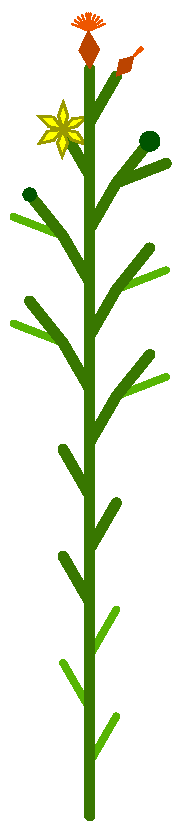
\includegraphics[scale=0.5]{MycelisMuralis50}} ~
	\subfloat[55]{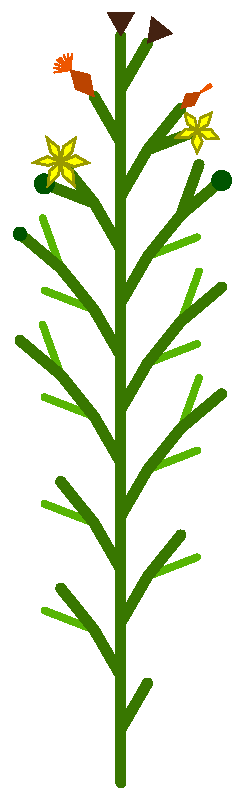
\includegraphics[scale=0.5]{MycelisMuralis55}} ~
	\subfloat[60]{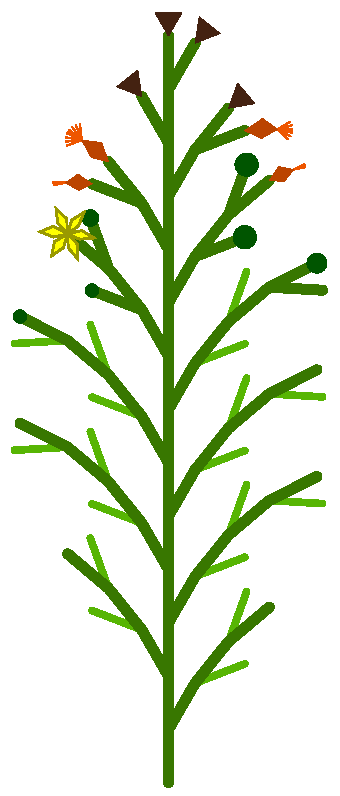
\includegraphics[scale=0.5]{MycelisMuralis60}} ~
	\subfloat[65]{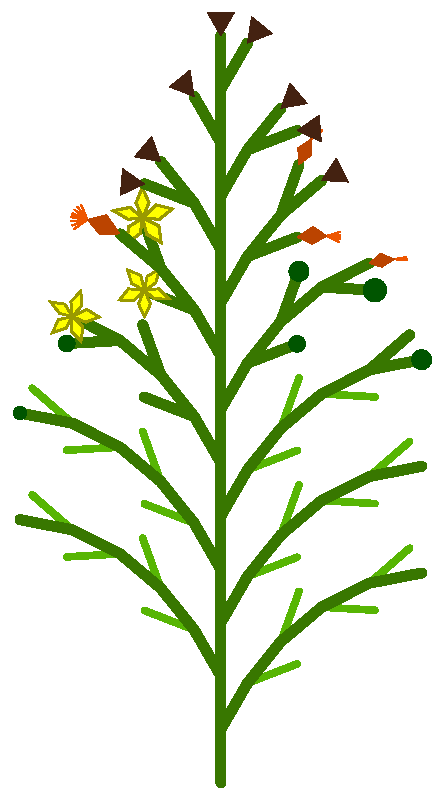
\includegraphics[scale=0.5]{MycelisMuralis65}} \\
	\subfloat[70]{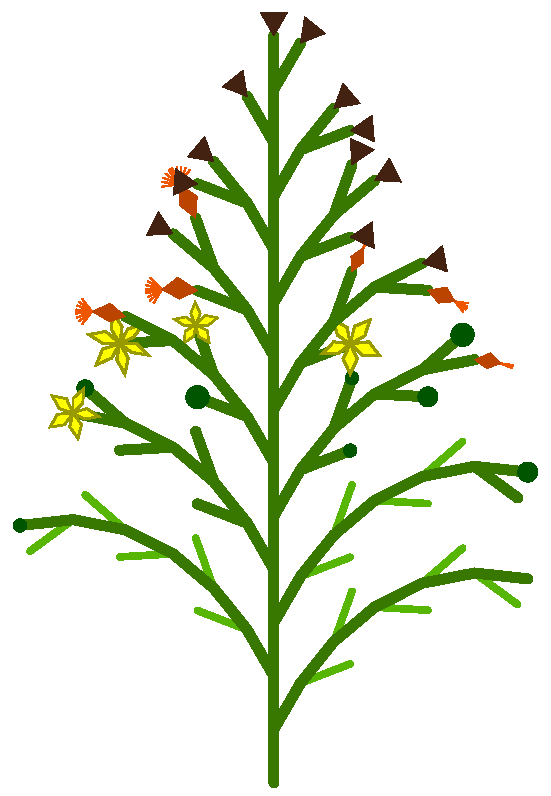
\includegraphics[scale=0.45]{MycelisMuralis70}} ~
	\subfloat[75]{
\includegraphics[scale=0.45]{MycelisMuralis75}} ~
	\subfloat[80]{
\includegraphics[scale=0.45]{MycelisMuralis80}} \\
	\subfloat[90]{
\includegraphics[scale=0.44]{MycelisMuralis90}} ~
	\subfloat[98]{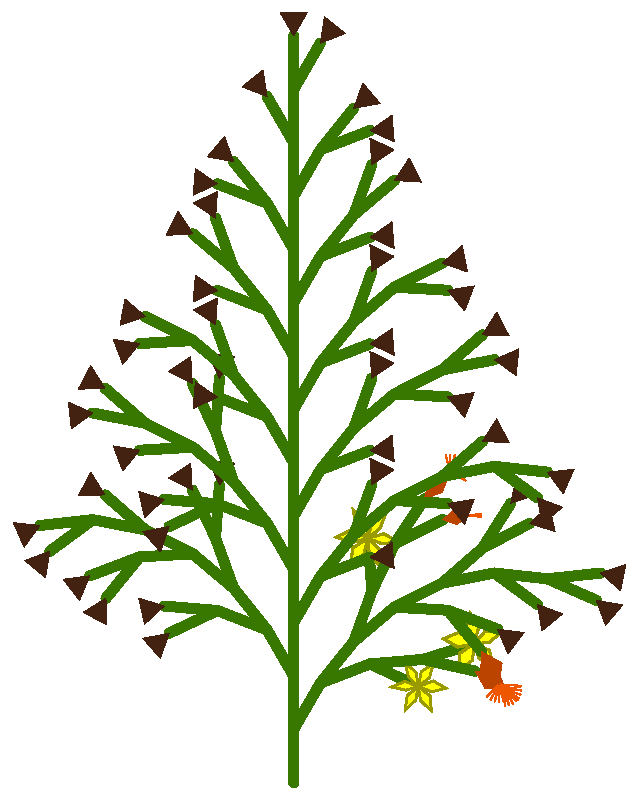
\includegraphics[scale=0.44]{MycelisMuralis98}} ~
	\subfloat[110]{
\includegraphics[scale=0.44]{MycelisMuralis110}}
	\caption{Some iterations of the \emph{MycelisMuralis} \lsystem}
	\label{fig:MycelisMuralis}
\end{figure}





